\begin{exercise}{5.6}
    Consider the eigenvalues of the operators, $L_1$, $L_2$, and $L_3$, where $L_1 u = u_x$, $L_2 u = -\alpha u_{xx}$, $\alpha = 1.0 e^{-5}$, and $L_3 = L_1 + L_2$, with homogeneous Dirichlet conditions.
    For which of the operators are the eigenvalues positive and real?
    Repeat the exercise with $L_1 = x u_x$.
\end{exercise}

\begin{solution}{5.6}
    Here, I assume that the domain is $[0, 1]$, and the boundary conditions are $u(0) = u(1) = 0$.
    Solving for the eigenvalues for the first operators is not terribly difficult, although it is a bit tedious.
    Instead, we will use the finite element method.

    With the eigenvalue problem $L u = \lambda u$, we have the associated weak form
    \begin{equation*}
        \int_0^1 L u \, v \, \diff x = \lambda \int_0^1 u \, v \, \diff x,
    \end{equation*}
    where $L$ is one of the operators $L_1$, $L_2$, or $L_3$.
    For the first operator, we then have
    \begin{equation*}
        \int_0^1 u_x \, v \, \diff x = \lambda \int_0^1 u \, v \, \diff x.
    \end{equation*}
    For $L_2$ we have
    \begin{equation*}
        \int_{0}^{1} -\alpha u_{xx} \, v \, \diff x = \lambda \int_{0}^{1} u \, v \, \diff x,
    \end{equation*}
    however, we can integrate by parts to get
    \begin{equation*}
        \int_{0}^{1} \alpha u_x \, v_x \, \diff x = \lambda \int_{0}^{1} u \, v \, \diff x.
    \end{equation*}
    Finally, for $L_3$ we have
    \begin{equation*}
        \int_{0}^{1} (u_x - \alpha u_{xx}) \, v \, \diff x = \lambda \int_{0}^{1} u \, v \, \diff x,
    \end{equation*}
    which again can be integrated by parts to get
    \begin{equation*}
        \int_{0}^{1} u_x \, v  + \alpha u_x \, v_x \, \diff x = \lambda \int_{0}^{1} u \, v \, \diff x.
    \end{equation*}

    This is implemented in \texttt{eigs.py}, resulting in the eigenvalues shown in \cref{fig:eigenvalues}.
    Atleast according to my implementation, the only operator with positive real eigenvalues is $L_2$.

    \begin{figure}[ht]
        \centering
        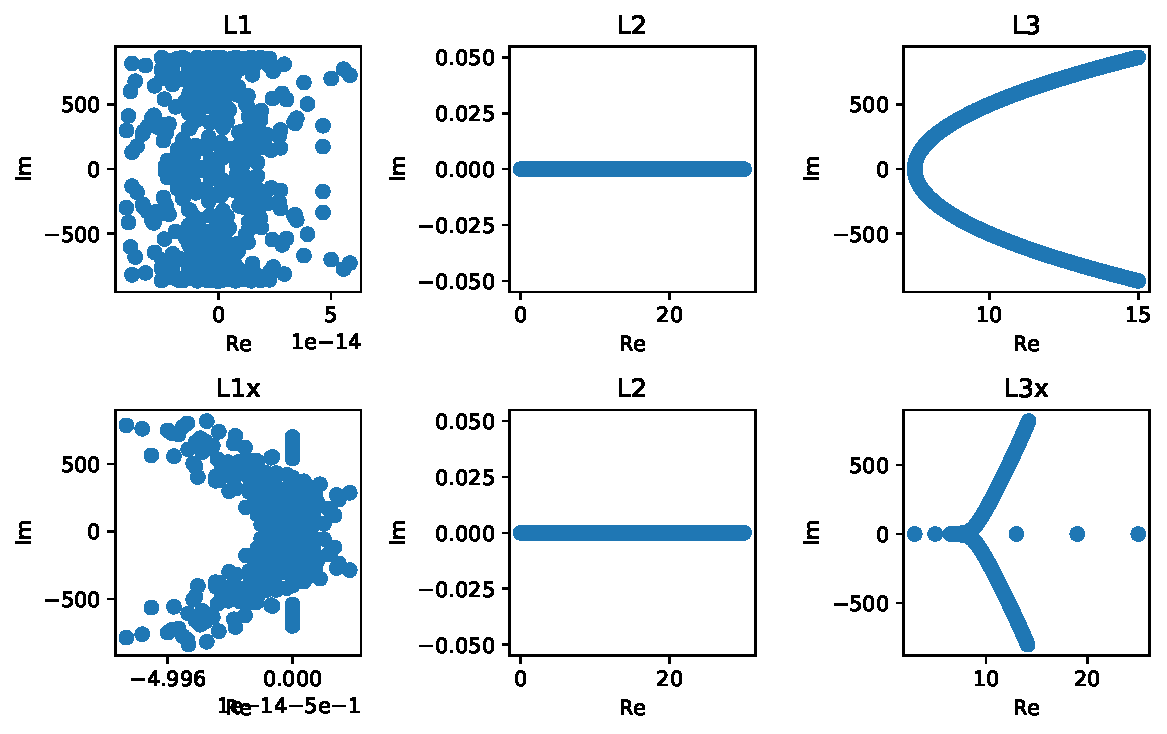
\includegraphics[width=0.8\textwidth]{eigs.pdf}
        \caption{Eigenvalues for the operators $L_1$, $L_2$, and $L_3$ with homogeneous Dirichlet conditions.\label{fig:eigenvalues}}
    \end{figure}
\end{solution}

\begin{exercise}{6.1}
    Show that the conditions in \cref{eq:6.15,eq:6.16,eq:6.17} are satisfied for $V_h = H^1_0$ and $Q_h = L^2$.
\end{exercise}

\begin{solution}{6.1}
    For this exercise we are considering Stokes problem, wherein we want to find $u_h \in V_h$ and $p_h \in Q_h$ such that
    \begin{equation}
        \begin{split}
            a(u_h, v_h) + b(p_h, v_h) &= f(v_h), \quad \forall v_h \in V_h, \\
            b(q_h, u_h) &= 0, \quad \forall q_h \in Q_h,
        \end{split}
    \end{equation}
    where
    \begin{equation}
        \begin{split}
            a(u, v) &= \int_{\Omega} \nabla u : \nabla v \diff x, \\
            b(p, v) &= \int_{\Omega} p \, \nabla \cdot v \diff x, \\
            f(v) &= \int_{\Omega} f \, v \diff x + \int_{\Omega_N} h \, v \diff s.
        \end{split}
    \end{equation}
    The conditions to show are then
    \begin{align}
        \text{\small Boundedness of $a$:}
        && \quad a(u_h, v_h) &\leq C_1 \norm{u_h}_{V_h} \norm{v_h}_{V_h},
        & \forall u_h, v_h \in V_h,
        \tag{6.15} \label{eq:6.15}
        \\
        \text{\small Boundedness of $b$:}
        && \quad b(q_h, u_h) &\leq C_2 \norm{q_h}_{Q_h} \norm{u_h}_{V_h},
        & \forall u_h \in V_h, q_h \in Q_h,
        \tag{6.16} \label{eq:6.16}
        \\
        \text{\small Coercivity of $a$:}
        && \quad a(u_h, u_h) &\geq C_3 \norm{u_h}_{V_h}^2,
        & \forall u_h \in Z_h,
        \tag{6.17} \label{eq:6.17}
    \end{align}
    where $Z_h = \{ u_h \in V_h \mid b(u_h, q_h) = 0, \, \forall q_h \in Q_h \}$.

    For \cref{eq:6.15}, we have
    \begin{equation}
        a(u_h, v_h) = \int_{\Omega} \nabla u_h : \nabla v_h \diff x,
    \end{equation}
    which by the Cauchy-Schwarz inequality is bounded by
    \begin{equation}
        a(u_h, v_h) \leq \norm{\nabla u_h}_{L^2} \norm{\nabla v_h}_{L^2} = \abs{u_h}_{H^1} \abs{v_h}_{H^1}.
    \end{equation}
    As we have previously shown that the $H^1$ semi-norm is equivalent to the $H^1$ norm, \cref{eq:6.15} is satisfied.

    For \cref{eq:6.16}, we have
    \begin{equation}
        b(q_h, u_h) = \int_{\Omega} q_h \, \nabla \cdot u_h \diff x,
    \end{equation}
    which by the Cauchy-Schwarz inequality is bounded by
    \begin{equation}
        b(q_h, u_h) \leq \norm{q_h}_{L^2} \norm{\nabla \cdot u_h}_{L^2}.
    \end{equation}
    We already have $\norm{q_h}_{L^2}$ as desired, and we now need to relate $\norm{\nabla \cdot u_h}_{L^2}$ to $\norm{\nabla u_h}_{L^2}$.
    We have
    \begin{align*}
        \abs{\nabla \cdot u(x)}^2
        &= \abs*{\sum_{i = 0}^{d} \frac{\partial u_i}{\partial x_i}(x)}^2
        \leq \left(
            \sum_{i = 0}^{d} 1
        \right) \left(
            \sum_{i = 0}^{d} \left( \frac{\partial u_i}{\partial x_i}(x) \right)^2
        \right)
        = d \sum_{i = 0}^{d} \left( \frac{\partial u_i}{\partial x_i}(x) \right)^2.
    \end{align*}
    Therefore,
    \begin{align*}
        \norm{\nabla \cdot u_h}_{L^2}^2
        &= \int_{\Omega} \abs{\nabla \cdot u_h}^2 \diff x
        \leq d \int_{\Omega} \sum_{i = 0}^{d} \left(
            \frac{\partial u_i}{\partial x_i}
        \right)^2 \diff x \\
        &\leq d \int_{\Omega} \sum_{i = 0}^{d} \sum_{j = 0}^{d} \left(
            \frac{\partial u_i}{\partial x_j}
        \right)^2 \diff x
        = d \int_{\Omega} \abs{\nabla u_h}^2 \diff x \\
        &= d \norm{\nabla u_h}_{L^2}^2.
    \end{align*}
    Using this, we have
    \begin{equation}
        b(q_h, u_h) \leq \sqrt{d} \norm{q_h}_{L^2} \norm{\nabla u_h}_{L^2},
    \end{equation}
    and as such \cref{eq:6.16} is satisfied.

    For \cref{eq:6.17}, we have
    \begin{equation}
        a(u_h, u_h)
        = \int_{\Omega} \nabla u_h : \nabla u_h \diff x
        = \norm{\nabla u_h}_{L^2}^2 = \abs{u_h}_{H^1}^2.
    \end{equation}
    As we have previously shown that the $H^1$ semi-norm is equivalent to the $H^1$ norm, \cref{eq:6.17} is satisfied.

    We have thus shown that the conditions in \cref{eq:6.15,eq:6.16,eq:6.17} are satisfied for $V_h = H^1_0$ and $Q_h = L^2$.
\end{solution}

\newpage

\begin{comment}

\begin{exercise}{5.6}
    Consider the eigenvalues of the operators, $L_1$, $L_2$, and $L_3$, where $L_1 u = u_x$, $L_2 u = -\alpha u_{xx}$, $\alpha = 1.0 e^{-5}$, and $L_3 = L_1 + L_2$, with homogeneous Dirichlet conditions.
    For which of the operators are the eigenvalues positive and real?
    Repeat the exercise with $L_1 = x u_x$.
\end{exercise}

\begin{comment}
    \begin{solution}{4.6}
    For this exercise, I'm assuming that the domain is $[0, 1]$.
    For $L_1$, the eigenfunctions are of the from
    \begin{equation}
        u(x) = C e^{\lambda x},
    \end{equation}
    as we then have
    \begin{equation}
        L_1 C e^{\lambda x} = \frac{\partial}{\partial x} C e^{\lambda x} = C \lambda e^{\lambda x}.
    \end{equation}
    For the boundary conditions, we have $u(0) = u(1) = 0$, which gives us
    \begin{equation}
        C e^{\lambda \cdot 0} = C e^0 = C
    \end{equation}
    and
    \begin{equation}
        e^{\lambda \cdot 1} = C e^{\lambda},
    \end{equation}
    which gives us the trivial solution $C = 0$ and $u(x) = 0$, for all $\lambda$.

    For $L_2$, we consider first the operator $\frac{\partial^2}{\partial x^2}$.
    The eigenfunctions of this operator are loosely of the form
    \begin{equation}
        u(x) = e^{i x},
    \end{equation}
    as then
    \begin{equation}
        \frac{\partial^2}{\partial x^2} e^{i x} = -i^2 e^{i x} = -e^{i x}.
    \end{equation}
    In order to get the factor $\alpha$, we need to adjust the exponent such that we have
    \begin{equation}
        u(x) = e^{i \sqrt{\alpha} x}.
    \end{equation}
\end{solution}
% \end{comment}

\begin{solution}{5.6}
    For this exercise, let the domain be $[0, 1]$ for simplicity.
    For the first part of the exercise, we are seeking solutions to
    \begin{equation}
        u_x = \lambda u,
    \end{equation}
    for which the solutions are
    \begin{equation}
        u(x) = C e^{\lambda x}.
    \end{equation}
    The boundary conditions are $u(0) = u(1) = 0$, which gives us that $C = 0$, and thus $u(x) = 0$ for all $\lambda$.

    For the second part of the exercise, we are seeking solutions to
    \begin{equation}
        -\alpha u_{xx} = \lambda u,
    \end{equation}
    or equivalently
    \begin{equation}
        -u_{xx} = \tfrac{\lambda}{\alpha} u.
    \end{equation}
    As the second derivative is a scaled version of the function itself, with opposite sign, we can guess that the solutions are of the form
    \begin{equation}
        u(x) = \sin(C x)
        \quad \text{or} \quad
        u(x) = \cos(C x).
    \end{equation}
    As the boundary conditions are homogeneous Dirichlet conditions, we can see that the sine function is the only one that satisfies the boundary conditions, for $C = k \pi$, $k = 0, 1, 2, \ldots$.
    Taking the double derivative of the sine function, we get
    \begin{equation}
        -u_{xx} = (k \pi)^2 \sin(k \pi x),
    \end{equation}
    and hence
    \begin{equation}
        \tfrac{\lambda}{\alpha} = (k \pi)^2 \implies \lambda = \alpha (k \pi)^2.
    \end{equation}
    As $\alpha > 0$, we see that the eigenvalues are positive and real for $L_2$, for $k \geq 1$.

    For $L_3$, we are looking for a solution
    \begin{equation}
        u_x - \alpha u_{xx} = \lambda u.
    \end{equation}
    Recalling back to videregående ODE solving, we can guess that the solution is of the form
    \begin{equation}
        u(x) = e^{rx},
    \end{equation}
    which gives the equation
    \begin{equation}
        -\alpha r^2 + r - \lambda = 0.
    \end{equation}
    Recalling the abc-formula, we then have the solutions
    \begin{align}
        r &=
        \frac{-1 \pm \sqrt{1 - 4 \alpha \lambda}}{-2 \alpha}
        = \frac{1 \mp \sqrt{1 - 4 \alpha \lambda}}{2 \alpha}.
    \end{align}
    For $1 - 4 \alpha \lambda > 0$, we have two real roots, however they only permit the trivial solution.
    For $1 - 4 \alpha \lambda = 0$, we have one real root, $r = 1 / 2\alpha$, which gives us a solution of the form
    \begin{equation}
        (C_1 + C_2 x) e^{x / 2\alpha},
    \end{equation}
    however for the boundary conditions, we must have $C_1 = C_2 = 0$, and hence the only solution is the trivial one.

    Finally, for $1 - 4 \alpha \lambda < 0$, we have two complex roots
    \begin{equation}
        r = \frac{1}{2\alpha} \pm i \frac{\sqrt{4 \alpha \lambda - 1}}{2\alpha},
    \end{equation}
    which gives us a solution of the form
    \begin{equation}
        e^{x / 2\alpha} \left(
            C_1 \cos\left(\frac{\sqrt{4 \alpha \lambda - 1}}{2\alpha} x\right)
            + C_2 \sin\left(\frac{\sqrt{4 \alpha \lambda - 1}}{2\alpha} x\right)
        \right).
    \end{equation}
    At $x = 0$, we have
    \begin{equation}
        e^{0} \left(
            C_1 \cos\left(\frac{\sqrt{4 \alpha \lambda - 1}}{2\alpha} \cdot 0 \right)
            + C_2 \sin\left(\frac{\sqrt{4 \alpha \lambda - 1}}{2\alpha} \cdot 0 \right)
        \right),
    \end{equation}
    such that we must have $C_1 = 0$.
    At $x = 1$, we have
    \begin{equation}
        e^{1 / 2\alpha} \left( C_2 \sin\left(\frac{\sqrt{4 \alpha \lambda - 1}}{2\alpha}\right) \right) = 0,
    \end{equation}
    which is valid when $\frac{\sqrt{4 \alpha \lambda - 1}}{2\alpha} = k \pi$, $k = 0, 1, 2, \ldots$.
    This gives us the eigenvalues
    \begin{align*}
        \frac{\sqrt{4 \alpha \lambda - 1}}{2\alpha} &= k \pi \\
        4 \alpha \lambda - 1 &= (2\alpha k \pi)^2 \\
        \lambda &= \frac{(2 \alpha k \pi)^2 + 1}{4 \alpha} \\
        \lambda &= \alpha (k \pi)^2 + \frac{1}{4 \alpha},
    \end{align*}
    which are always positive and real.

    Changing $L_1$ to $x u_x$, we have the equation
    \begin{equation}
        x u_x = \lambda u \implies u_x = \frac{\lambda}{x} u.
    \end{equation}
    As far as I can see, the monomials satisfy the equation, as
    \begin{equation}
        u_x = \frac{\partial}{\partial x} x^n = n x^{n - 1} = \frac{n}{x} x^n = \frac{n}{x} u.
    \end{equation}
    Looking even closer, we see that we do not even need to restrict ourselves the monomials, but can rather have
    \begin{equation}
        u(x) = C x^\lambda,
        \quad \text{for }
        \lambda \in \mathbb{R},
    \end{equation}
    however as zero is included in the domain, we require that $\lambda > 0$.
    At $x = 0$ we have $u(0) = 0$, while we at $x = 1$ have
    \begin{equation}
        u(1) = C,
    \end{equation}
    and as such we sadly only have the trivial solution $u(x) = 0$ for all $\lambda$.

    I have no clue as to how to find the eigenvalues for $L_3$ when $L_1 = x u_x$.

    With this new $L_1$, we have that
    \begin{equation}
        L_3 u = x u_x - \alpha u_{xx},
    \end{equation}

    \begin{equation}
        \lambda u - x u_x + \alpha u_{xx} = 0.
    \end{equation}
\end{solution}

\begin{exercise}{6.1}
    Show that the conditions in \cref{eq:6.15,eq:6.16,eq:6.17} are satisfied for $V_h = H^1_0$ and $Q_h = L^2$.
\end{exercise}

\begin{solution}{6.1}
    For this exercise we are considering Stokes problem, wherein we want to find $u_h \in V_h$ and $p_h \in Q_h$ such that
    \begin{equation}
        \begin{split}
            a(u_h, v_h) + b(p_h, v_h) &= f(v_h), \quad \forall v_h \in V_h, \\
            b(q_h, u_h) &= 0, \quad \forall q_h \in Q_h,
        \end{split}
    \end{equation}
    where
    \begin{equation}
        \begin{split}
            a(u, v) &= \int_{\Omega} \nabla u : \nabla v \diff x, \\
            b(p, v) &= \int_{\Omega} p \, \nabla \cdot v \diff x, \\
            f(v) &= \int_{\Omega} f \, v \diff x + \int_{\Omega_N} h \, v \diff s.
        \end{split}
    \end{equation}
    The conditions to show are then
    \begin{align}
        \text{\small Boundedness of $a$:}
        && \quad a(u_h, v_h) &\leq C_1 \norm{u_h}_{V_h} \norm{v_h}_{V_h},
        & \forall u_h, v_h \in V_h,
        \tag{6.15} \label{eq:6.15}
        \\
        \text{\small Boundedness of $b$:}
        && \quad b(q_h, u_h) &\leq C_2 \norm{q_h}_{Q_h} \norm{u_h}_{V_h},
        & \forall u_h \in V_h, q_h \in Q_h,
        \tag{6.16} \label{eq:6.16}
        \\
        \text{\small Coercivity of $a$:}
        && \quad a(u_h, u_h) &\geq C_3 \norm{u_h}_{V_h}^2,
        & \forall u_h \in Z_h,
        \tag{6.17} \label{eq:6.17}
    \end{align}
    where $Z_h = \{ u_h \in V_h \mid b(u_h, q_h) = 0, \, \forall q_h \in Q_h \}$.

    For \cref{eq:6.15}, we have
    \begin{equation}
        a(u_h, v_h) = \int_{\Omega} \nabla u_h : \nabla v_h \diff x,
    \end{equation}
    which by the Cauchy-Schwarz inequality is bounded by
    \begin{equation}
        a(u_h, v_h) \leq \norm{\nabla u_h}_{L^2} \norm{\nabla v_h}_{L^2} = \abs{u_h}_{H^1} \abs{v_h}_{H^1}.
    \end{equation}
    As we have previously shown that the $H^1$ semi-norm is equivalent to the $H^1$ norm, \cref{eq:6.15} is satisfied.

    For \cref{eq:6.16}, we have
    \begin{equation}
        b(q_h, u_h) = \int_{\Omega} q_h \, \nabla \cdot u_h \diff x,
    \end{equation}
    which by the Cauchy-Schwarz inequality is bounded by
    \begin{equation}
        b(q_h, u_h) \leq \norm{q_h}_{L^2} \norm{\nabla \cdot u_h}_{L^2}.
    \end{equation}
    We already have $\norm{q_h}_{L^2}$ as desired, and we now need to relate $\norm{\nabla \cdot u_h}_{L^2}$ to $\norm{\nabla u_h}_{L^2}$.
    We have
    \begin{align*}
        \abs{\nabla \cdot u(x)}^2
        &= \abs*{\sum_{i = 0}^{d} \frac{\partial u_i}{\partial x_i}(x)}^2
        \leq \left(
            \sum_{i = 0}^{d} 1
        \right) \left(
            \sum_{i = 0}^{d} \left( \frac{\partial u_i}{\partial x_i}(x) \right)^2
        \right)
        = d \sum_{i = 0}^{d} \left( \frac{\partial u_i}{\partial x_i}(x) \right)^2.
    \end{align*}
    Therefore,
    \begin{align*}
        \norm{\nabla \cdot u_h}_{L^2}^2
        &= \int_{\Omega} \abs{\nabla \cdot u_h}^2 \diff x
        \leq d \int_{\Omega} \sum_{i = 0}^{d} \left(
            \frac{\partial u_i}{\partial x_i}
        \right)^2 \diff x \\
        &\leq d \int_{\Omega} \sum_{i = 0}^{d} \sum_{j = 0}^{d} \left(
            \frac{\partial u_i}{\partial x_j}
        \right)^2 \diff x
        = d \int_{\Omega} \abs{\nabla u_h}^2 \diff x \\
        &= d \norm{\nabla u_h}_{L^2}^2.
    \end{align*}
    Using this, we have
    \begin{equation}
        b(q_h, u_h) \leq \sqrt{d} \norm{q_h}_{L^2} \norm{\nabla u_h}_{L^2},
    \end{equation}
    and as such \cref{eq:6.16} is satisfied.

    For \cref{eq:6.17}, we have
    \begin{equation}
        a(u_h, u_h)
        = \int_{\Omega} \nabla u_h : \nabla u_h \diff x
        = \norm{\nabla u_h}_{L^2}^2 = \abs{u_h}_{H^1}^2.
    \end{equation}
    As we have previously shown that the $H^1$ semi-norm is equivalent to the $H^1$ norm, \cref{eq:6.17} is satisfied.

    We have thus shown that the conditions in \cref{eq:6.15,eq:6.16,eq:6.17} are satisfied for $V_h = H^1_0$ and $Q_h = L^2$.
\end{solution}
\end{comment}

\begin{exercise}{6.2}
    Show that the conditions in \cref{eq:6.15,eq:6.16,eq:6.17} are satisfied for Taylor--Hood and Mini discretizations. % chktex 8
    (Note that Crouzeix--Raviart is non-conforming so it is more difficult to prove these conditions for this case.) % chktex 8
\end{exercise}

\begin{solution}{6.2}
    The Taylor--Hood elements are defined by the basis functions % chktex 8
    \begin{equation}
        \begin{split}
            u &: N_i = a_i + b_i x + c_i y + d_i x y + e_i x^2 + f_i y^2, \\
            p &: L_i = k_i + l_i x + m_i y.
        \end{split}
    \end{equation}
    We then have
    \begin{align*}
        \nabla u &=
        \begin{bmatrix}
            b_i + d_i y + 2 e_i x \\
            c_i + d_i x + 2 f_i y
        \end{bmatrix},
        &
        \nabla \cdot u &= ?
        &
        \nabla p &=
        \begin{bmatrix}
            l_i \\
            m_i
        \end{bmatrix}.
    \end{align*}

    \begin{equation}
        u_h = \sum_{i = 1}^{N} u_i N_i,
    \end{equation}
\end{solution}